% ===== Page 58 =====
\begin{theorem}
\leavevmode\origpage{58}Let $A$ be an $n\times n$ matrix with $n$ distinct eigenvalues, $\lambda_1,\lambda_2,\dots,\lambda_n$ where $\lambda_i\neq\lambda_j$ when $i\neq j$. Then
\[
\begin{array}{rccccccc@{\;}l}
\C^n = & \Null(A-\lambda_1 I) & \oplus & \Null(A-\lambda_2 I) & \oplus\cdots\oplus & \Null(A-\lambda_n I) & & & \\
 & \Span\{e_1\} & & \Span\{e_2\} & & \Span\{e_n\} & & & \\[4pt]
 & 1 & + & 1 & +\cdots+ & 1 & = & n &
\end{array}
\]
\end{theorem}
Since $\Null(A-\lambda_i I)$ is invariant under $A$, \key{$A$ has a diagonal representation}:
\[
\bar A=\begin{bmatrix}\lambda_1 & & & 0\\ & \lambda_2 & & \\ & & \ddots & \\ 0 & & & \lambda_n\end{bmatrix},
\qquad \bar A = P^{-1}AP \quad\text{where } P=\big[\,e_1 \mid e_2 \mid \dots \mid e_n\,\big].
\]
% corrected: notes label the diagonal matrix "A"; it is \bar A = P^{-1}AP

\paragraph{Linear independence of $e_1,\ e_2,\ \dots,\ e_n$.}
Suppose
\[ \alpha_1 e_1+\alpha_2 e_2+\dots+\alpha_n e_n = 0 \]
and use
\[ (A-\lambda_i I)e_j = Ae_j-\lambda_i e_j = \lambda_j e_j - \lambda_i e_j = (\lambda_j-\lambda_i)e_j . \]
Multiply with $(A-\lambda_1 I)$, then with $(A-\lambda_2 I)$, and so on:
\begin{align*}
\times(A-\lambda_1 I):&\quad 0 + (\lambda_2-\lambda_1)\alpha_2 e_2 + \alpha_3(\lambda_3-\lambda_1)e_3 + \dots + \alpha_n(\lambda_n-\lambda_1)e_n = 0\\
\times(A-\lambda_2 I):&\quad 0+0+\alpha_3(\lambda_3-\lambda_1)(\lambda_3-\lambda_2)e_3+\dots+\alpha_n(\lambda_n-\lambda_1)(\lambda_n-\lambda_2)e_n = 0\\
&\quad\ \vdots\\
&\quad \alpha_n\underbrace{(\lambda_n-\lambda_1)(\lambda_n-\lambda_2)\cdots(\lambda_n-\lambda_{n-1})}_{\neq 0}\,\underbrace{e_n}_{\neq 0} = 0
\quad\Longrightarrow\quad \alpha_n = 0 \;\Longrightarrow\; \forall \alpha_i = 0
\end{align*}
\explain{The product is nonzero for distinct eigenvalues (this case), and $e_n$ is nonzero.}
\begin{insight}[Completing the argument]
After the $n-1$ multiplications only the $e_n$-term survives, so $\alpha_n=0$. The original relation then has only the terms $e_1,\dots,e_{n-1}$; repeating the procedure with the factors $(A-\lambda_1I),\dots,(A-\lambda_{n-2}I)$ gives $\alpha_{n-1}=0$, and so on; hence all $\alpha_i=0$. Thus $\{e_1,\dots,e_n\}$ is a set of $n$ linearly independent vectors in $\C^n$, i.e.\ a basis, and each $\Null(A-\lambda_iI)$ is exactly one-dimensional (it is at least $1$-dimensional, and the dimensions cannot add up to more than $n$). This proves the direct sum in the theorem.
\end{insight}

\sep
\[
P=\big[\,e_1\mid e_2\mid\dots\mid e_n\,\big], \qquad \bar A = P^{-1}AP \;\Rightarrow\; P\bar A = AP
\]
\begin{align*}
\big[\,e_1\mid e_2\mid\dots\mid e_n\,\big]
\begin{bmatrix}\lambda_1 & 0 & \cdots & 0\\ 0 & \lambda_2 & & \vdots\\ \vdots & & \ddots & \vdots\\ 0 & \cdots & \cdots & \lambda_n\end{bmatrix}
&= A\big[\,e_1\mid e_2\mid\dots\mid e_n\,\big]\\
&= \big[\,Ae_1\mid Ae_2\mid\dots\mid Ae_n\,\big]\\
&= \big[\,\lambda_1 e_1 \;\; \lambda_2 e_2 \;\; \dots\;\; \lambda_n e_n\,\big]
\end{align*}

\begin{keybox}
\noindent\hfil$\displaystyle\begin{aligned}
\therefore\ \text{Distinct eigenvalues} &\;\Rightarrow\; \text{Diagonalizable matrix}\\
&\;\Rightarrow\; \text{we can find $P$ matrix \& $\bar A$}\\[2pt]
\text{Distinct eigenvalues} &\;\not\Leftarrow\; \text{Diagonalizable}
\end{aligned}$\hfil\par\smallskip
Contrapositive ($p\Rightarrow q \;\equiv\; \bar q\Rightarrow \bar p$):\quad Non-diagonalizable $\;\Rightarrow\;$ repeated eigenvalues.
\end{keybox}
Two diagonal matrices with repeated eigenvalues:
\[
A=\bmat{1&0&0\\0&1&0\\0&0&1},\quad d(s)=(s-1)^3
\qquad\qquad
\bmat{2&0&0\\0&2&0\\0&0&1}
\]
\explain{Diagonal, but repeated eigenvalues.}
Both matrices are already diagonal (so trivially diagonalizable with $P=I$), yet their eigenvalues are repeated: this is why the converse implication fails.

% ===== Page 59 =====
\section{Characteristic and Minimal Polynomials}\label{sec:polys}
\syllabusweek{Week 10 --- Cayley--Hamilton theorem, characteristic and minimal polynomials}
\subsection{Similar Matrices and the Characteristic Polynomial}\label{ss:charpoly}
\origpage{59}%
% (a rotated personal side note in Turkish in the margin, unrelated to the material, is omitted)
\key{Similar matrices have the same characteristic polynomial:}
\begin{align*}
\bar d(s) &= \det(sI-\bar A)\\
&= \det(sI-P^{-1}AP)\\
&= \det(sP^{-1}P-P^{-1}AP) = \det\big(P^{-1}(sI-A)P\big)\\
&= \det P^{-1}\,\det(sI-A)\,\det P\\
&= \frac{1}{\cancel{\det P}}\cdot\det(sI-A)\cdot\cancel{\det P}\\
&= \det(sI-A) = d(s)
\end{align*}
\explain{Uses $\det(XY)=\det X\det Y$ and $\det P^{-1}=1/\det P$. Hence \key{similar matrices have the same eigenvalues} (with the same algebraic multiplicities); in particular the eigenvalues of $A$ are the diagonal entries of $\bar A$.}

\begin{example}
\[
A=\bmat{1&0&0\\-1&2&1\\0&0&3},\qquad sI-A=\bmat{s-1&0&0\\1&s-2&-1\\0&0&s-3}
\]
% corrected: notes had A_{31}=1, inconsistent with sI-A (entry 0) and with all following computations (A-lambda_i I, null spaces, the check AP); A_{31}=0 is meant
\[
\det(sI-A)=(s-1)\begin{vmatrix}s-2&-1\\0&s-3\end{vmatrix} = (s-1)(s-2)(s-3)=0
\quad\Rightarrow\quad \lambda=1,\ \ \lambda=2,\ \ \lambda=3
\]
\begin{align*}
A-\lambda_1 I &= \bmat{0&0&0\\-1&1&1\\0&0&2}, & \Null(A-\lambda_1 I)&=\Span\left\{\bmat{1\\1\\0}\right\}\\
A-\lambda_2 I &= \bmat{-1&0&0\\-1&0&1\\0&0&1}, & \Null(A-\lambda_2 I)&=\Span\left\{\bmat{0\\1\\0}\right\}\\
A-\lambda_3 I &= \bmat{-2&0&0\\-1&-1&1\\0&0&0}, & \Null(A-\lambda_3 I)&=\Span\left\{\bmat{0\\1\\1}\right\}
\end{align*}
\begin{align*}
P&=\bmat{1&0&0\\1&1&1\\0&0&1}, & \bar A&=\bmat{1&0&0\\0&2&0\\0&0&3}=P^{-1}AP\\
P&=\bmat{0&0&1\\1&1&1\\1&0&0}, & \bar A&=\bmat{3&0&0\\0&2&0\\0&0&1}
\end{align*}
Check for the second choice ($P\bar A=AP$):
\begin{align*}
\bmat{0&0&1\\1&1&1\\1&0&0}\overbrace{\bmat{3&0&0\\0&2&0\\0&0&1}}^{\bar A} &= A\bmat{0&0&1\\1&1&1\\1&0&0}
= \bmat{0&0&1\\3&2&1\\3&0&0}
\end{align*}
\explain{Both sides agree, so $P^{-1}AP=\bar A$. Reordering the eigenvectors in $P$ only reorders the eigenvalues on the diagonal of $\bar A$.}
\end{example}

\sep
\paragraph{Characteristic polynomial and equation.}
\[
A=\bmat{2&1\\1&2},\qquad
d(s)=\det(sI-A)=\left|\bmat{s-2&-1\\-1&s-2}\right|
\]
\begin{alignat*}{2}
d(s)&=s^2-4s+3 &\qquad&\Rightarrow\ \text{\term{charac.\ poly.}}\\
d(s)&=0 &&\Rightarrow\ \text{\term{charac.\ eqn.}}
\end{alignat*}
\begin{align*}
d(A)=A^2-4A+3I &= \bmat{2&1\\1&2}\bmat{2&1\\1&2}-4\bmat{2&1\\1&2}+3\bmat{1&0\\0&1}\\
&= \bmat{5&4\\4&5}-\bmat{8&4\\4&8}+\bmat{3&0\\0&3}=\bmat{0&0\\0&0}
\end{align*}
\[
\underline{\underline{d(A)=0_{n\times n}}}
\]

% ===== Page 60 =====
\subsection{The Cayley--Hamilton Theorem}\label{ss:cht}
\begin{theorem}[Cayley--Hamilton, CHT]
\leavevmode\origpage{60}\key{Every $n\times n$ matrix satisfies its characteristic equation.}
\[ \therefore\; d(A)=0_{n\times n} \]
\end{theorem}
\begin{align*}
d(s)&= s^n+d_1s^{n-1}+d_2s^{n-2}+\dots+d_{n-1}s+d_n\\
d(A)&= A^n+d_1A^{n-1}+d_2A^{n-2}+\dots+d_{n-1}A+d_nI = 0\\
A^n &= -d_1A^{n-1}-\dots-d_{n-1}A-d_n\underbrace{I}_{A^0}
\end{align*}
\explain{$\Rightarrow$ among the powers $I,A,A^2,\dots$ we can have at most $n$ linearly independent matrices.}
\begin{remark}
CHT says that \key{$n^{\text{th}}$ and higher order powers of an $n\times n$ matrix can be written as a linear combination of its lower powers.}
\end{remark}
For the matrix $A$ above, $d(A)=0$ gives:
\begin{align*}
A^2-4A+3I=0 \;\Rightarrow\; A^2 &= 4A-3I\\[2pt]
A^3 &= AA^2 = A(4A-3I)=4A^2-3A = 4(4A-3I)-3A\\
&= 13A-12I
\end{align*}
The inverse follows in the same way:
\begin{align*}
A^2-4A+3I&=0\\
A-4I+3A^{-1}&=0 \qquad\text{(multiply by $A^{-1}$; $A$ is invertible since $d(0)=3\neq0$)}\\
A^{-1}&=-\frac{A}{3}+\frac{4I}{3}=\frac13\bmat{2&-1\\-1&2}
\end{align*}
% corrected: notes had "A - 4 + 3A^{-1} = 0" (identity matrix missing)
In general, every power $A^i$ ($i\ge n$) reduces to
\[
\therefore\; A^i = \alpha_1A^{n-1}+\alpha_2A^{n-2}+\dots+\alpha_{n-1}A+\alpha_nI
\]
% note: a stray "x" mark follows "A = 2x2" in the notes

\sep
\paragraph{The $2\times 2$ case.}
By CHT, for a $2\times2$ matrix every power is a combination of $A$ and $I$. To find the coefficients we use eigenvectors.
For an eigenpair $Ae_1=\lambda_1e_1$:
\begin{align*}
Ae_1&=\lambda_1e_1\\
A^2e_1&=A(Ae_1)=\lambda_1^2e_1\\
A^ie_1&=\lambda_1^ie_1\\
p(A)e_1&=p(\lambda_1)e_1
\end{align*}
\explain{For any polynomial $p$: $p(A)$ acts on an eigenvector as multiplication by $p(\lambda_1)$.}
\needspace{9\baselineskip}
\[
\boxed{A^i=\alpha_iA+\beta_i I}\qquad
\lambda_1=3\ (e_1),\qquad \lambda_2=1\ (e_2)
\]
\begin{align*}
\underbrace{A^ie_1}_{\lambda_1^ie_1}&=\alpha_i\underbrace{Ae_1}_{\lambda_1e_1}+\beta_i\underbrace{Ie_1}_{e_1}
&
A^ie_2&=\alpha_iAe_2+\beta_iIe_2\\
3^ie_1&=3\alpha_ie_1+\beta_ie_1
&
\lambda_2^ie_2&=\alpha_i\lambda_2e_2+\beta_ie_2\\
3^ie_1&=(3\alpha_i+\beta_i)e_1
&
\lambda_2^i&=\alpha_i\lambda_2+\beta_i
\end{align*}
Since $e_1,e_2\neq0$ we may compare coefficients; with $\lambda_2=1$ this gives
\begin{align*}
3\alpha_i+\beta_i&=3^i\\
\alpha_i+\beta_i&=1 \qquad (=1^i)
\end{align*}
\explain{Subtracting: $2\alpha_i=3^i-1$.}
\[
\alpha_i=\frac{3^i-1}{2},\qquad \beta_i=1-\alpha_i=1-\frac{3^i-1}{2}=\frac{3-3^i}{2}
\]
\[
\boxed{A^i=\frac{3^i-1}{2}A+\frac{3-3^i}{2}I}
\]
\begin{insight}[Check]
$i=0$: $0\cdot A+1\cdot I=I$; \ $i=1$: $A+0\cdot I=A$; \ $i=2$: $4A-3I$ (as found from CHT); \ $i=3$: $13A-12I$ (as above). The formula holds for every $i\ge0$, and in fact also for $i=-1$: $\frac{3^{-1}-1}{2}A+\frac{3-3^{-1}}{2}I=-\frac A3+\frac{4I}{3}=A^{-1}$.
\end{insight}

% ===== Page 61 =====
\subsection{The Minimal Polynomial}\label{ss:minpoly}
\origpage{61}Consider
\[
A=\bmat{2&0&0\\0&2&0\\0&0&1},\qquad d(s)=(s-2)^2(s-1)
\]
\begin{align*}
d(A)&=(A-2I)^2(A-I)\\
&=\bmat{0&0&0\\0&0&0\\0&0&-1}^2\bmat{1&0&0\\0&1&0\\0&0&0}\\
&=\bmat{0&0&0\\0&0&0\\0&0&1}\bmat{1&0&0\\0&1&0\\0&0&0}=\bmat{0&0&0\\0&0&0\\0&0&0}
\end{align*}
\begin{align*}
m(s)&=(s-2)(s-1)\\
m(A)&=(A-2I)(A-I)=\bmat{0&0&0\\0&0&0\\0&0&-1}\bmat{1&0&0\\0&1&0\\0&0&0}=0_{n\times n}
\end{align*}
% corrected: notes had m(A) = (A-2)(A-2)
\explain{Lowest order $\Rightarrow$ minimal polynomial. (A degree-1 monic $A-cI$ cannot vanish, since $A$ is not a multiple of $I$.)}

\begin{definition}
A \term{monic polynomial} is a polynomial whose coefficient of the highest-degree term is unity ($=1$).
\begin{itemize}[label=$\ast$]
\item $s^2+2s+3$ \quad (Monic)
\item $2s^2+2s+3$ \quad (Not monic)
\end{itemize}
\end{definition}
\begin{definition}
For an $n\times n$ matrix $A$, the \term{minimal polynomial} is the monic polynomial $m(s)$ with the smallest degree/order s.t.
\[ m(A)=0_{n\times n} \]
\end{definition}
\begin{theorem}
Given $A\in\C^{n\times n}$ let $m(s)$ be its minimal polynomial. Then
\begin{enumerate}[label=\Roman*)]
\item $m(s)$ is \key{unique};
\item \key{$m(s)$ divides $d(s)$} without any remainder: $\exists q(s)$ s.t.\ $d(s)=m(s)q(s)$;
% corrected: notes had "d(s) = m(s) d(s)" 
\item \key{every root of $d(s)$ is also a root of $m(s)$}.
\end{enumerate}
\end{theorem}

\paragraph{Candidates for $d(s)=(s-1)(s-2)^2$.}
\begin{itemize}[itemsep=2pt]
\item $\cancel{m(s)=(s-1)}$,\quad $\cancel{m(s)=(s-2)}$,\quad $\cancel{m(s)=(s-2)^2}$\newline {\small$\triangleright$} not possible, property III (a root of $d(s)$ is missing)
\item $\cancel{m(s)=(s-1)(s-3)}$,\quad $\cancel{m(s)=(s-2)^3}$\newline {\small$\triangleright$} not possible, property II (they do not divide $d(s)$)
\item $m(s)=(s-1)(s-2)\ \checkmark$\qquad $m(s)=(s-1)(s-2)^2\ \checkmark$\newline {\small$\triangleright$} the only possibilities (i.e.\ $d(s)=\underbrace{m(s)}_{(s-1)(s-2)}\underbrace{q(s)}_{(s-2)}$ or $q(s)=1$)
\end{itemize}
% corrected: in the notes this is a scattered list of crossed-out candidates with checkmarks
% (also next to crossed-out ones and next to "m(s)=(s-1)"); the last candidate is written
% "(s-1)(s-2)^1". By properties II and III the only possibilities are (s-1)(s-2) and (s-1)(s-2)^2.

\sep
In general, for $A\in\C^{n\times n}$:
\begin{align*}
d(s)&=(s-\lambda_1)^{r_1}(s-\lambda_2)^{r_2}\cdots(s-\lambda_k)^{r_k}, \qquad r_1+r_2+\dots+r_k=n\\
m(s)&=(s-\lambda_1)^{m_1}(s-\lambda_2)^{m_2}\cdots(s-\lambda_k)^{m_k}, \qquad \boxed{1\le m_i\le r_i}
\end{align*}
\explain{Lower bound ($1\le m_i$) by property III; upper bound by property II.}
% corrected: notes had upper bound "k"; r_i is meant (cf. page 63)

% ===== Page 62 =====
\begin{proof}
\leavevmode\origpage{62}% (a rotated personal doodle in the margin, unrelated to the material, is omitted)
\textbf{I)}\quad $p\to q \;\equiv\; p\wedge\bar q=\text{False} \;\stackrel{\Delta}{=}\;$ proof by contradiction.

Suppose $m(s)$ is not unique and minimal polynomial ($p\wedge\bar q$):
\begin{align*}
m_1(s) &\longrightarrow m_1(A)=0_{n\times n}\\
m_2(s) &\longrightarrow m_2(A)=0_{n\times n}\\
m_1(s)&\neq m_2(s)
\end{align*}
\begin{align*}
m_1(s)&=s^l+a_1s^{l-1}+\dots+a_l\\
m_2(s)&=s^l+b_1s^{l-1}+\dots+b_l, \qquad \exists i \text{ s.t. } a_i\neq b_i\\
r(s)&=m_1(s)-m_2(s)\\
r(s)&=(a_1-b_1)s^{l-1}+\dots+(a_l-b_l)\\
\bar r(s)&=\frac{r(s)}{\alpha}
\end{align*}
\explain{$r(s)\neq0$ since $m_1\neq m_2$, and $\deg r<l$ since the $s^l$ terms cancel; $\alpha$: coefficient of the highest order term $\Rightarrow$ $\bar r(s)$ is monic.}
\[ \deg\bar r(s) < \big(\deg m_1(s)=\deg m_2(s)\big) \]
\[
\bar r(A)=\frac{r(A)}{\alpha}=\frac{m_1(A)-m_2(A)}{\alpha}=\frac{0_{n\times n}-0_{n\times n}}{\alpha}=0_{n\times n}
\]
$\bar r(A)=0_{n\times n}$: we assumed $m_1,m_2$ are minimal, but found a monic $\bar r(s)$ of lower degree that also annihilates $A$ $\Rightarrow$ contradiction with minimality. Hence $m(s)$ is unique.

\sep
\textbf{II)}\quad Divide $d(s)$ by $m(s)$ (polynomial division):
\[ d(s)=m(s)q(s)+r(s), \qquad \deg r(s)<\deg m(s). \]
Suppose $r(s)\neq 0(s)$ (proof by contradiction). Then
\[ \exists\,\bar r(s)=\frac{r(s)}{\alpha}\text{ and }\bar r(s)\text{ is monic}\quad(\alpha:\text{ leading coefficient of } r(s)).\qquad \bar r(A)=\,? \]
% corrected: notes had "\bar r(s) = r(\alpha)/\alpha"; the division d = mq + r was only implicit
\[
\underbrace{\cancel{d(A)}}_{0_{n\times n}\text{ (CHT)}}=\underbrace{\cancel{m(A)}}_{0_{n\times n}}q(A)+r(A)\qquad\Rightarrow\qquad r(A)=0_{n\times n}\;\Rightarrow\;\bar r(A)=0_{n\times n}
\]
\explain{$\bar r$ is monic, annihilates $A$ and has lower degree than $m$: contradiction. So $r(s)=0$, i.e.\ $m(s)$ divides $d(s)$.}
\begin{insight}[The same argument in general]
The proof of II only used $d(A)=0$. Hence: \key{$m(s)$ divides every polynomial $p(s)$ with $p(A)=0$.}
\end{insight}

\sep
\textbf{III)}\quad Roots of $d(s)$ are eigenvalues of $A$.
\begin{align*}
&d(\lambda_i)=0\\
&Ae_i=\lambda_ie_i, \qquad e_i\neq 0\\
&m(\lambda_i)\stackrel{?}{=}0\\
&m(s)=s^l+a_1s^{l-1}+\dots+a_l\\
&m(A)=A^l+a_1A^{l-1}+\dots+a_lI=0_{n\times n}\\
&(A^l+a_1A^{l-1}+\dots+a_lI)e_i=0_{n\times 1}\\
&A^le_i+a_1A^{l-1}e_i+\dots+a_{l-1}Ae_i+a_le_i=0_{n\times1}\\
&(\lambda_i^l+a_1\lambda_i^{l-1}+\dots+a_{l-1}\lambda_i+a_l)\,\underbrace{e_i}_{\neq0}=0_{n\times1}\\
&\lambda_i^l+a_1\lambda_i^{l-1}+\dots+a_{l-1}\lambda_i+a_l=0 \;\Rightarrow\; m(\lambda_i)=0
\end{align*}
% corrected: notes had e_1 instead of e_i in two places, and a stray cancelled e_i inside the bracket
\explain{$A^je_i=\lambda_i^je_i$; a scalar times a nonzero vector is zero only if the scalar is zero.}
\[ \therefore\;\lambda_i \text{ is a root of } m(s). \qedhere \]
\end{proof}

% ===== Page 63 =====
\subsection{Minimal Polynomial and Null-Space Decomposition}\label{ss:minpoly-decomp}
\begin{keybox}
\origpage{63}\noindent\hfil$\displaystyle\begin{aligned}
\therefore\; d(s)&=(s-\lambda_1)^{r_1}(s-\lambda_2)^{r_2}\cdots(s-\lambda_k)^{r_k}\\
m(s)&=(s-\lambda_1)^{m_1}(s-\lambda_2)^{m_2}\cdots(s-\lambda_k)^{m_k}\\
&1\le m_i\le r_i, \qquad r_1+r_2+\dots+r_k=n
\end{aligned}$\hfil
\end{keybox}

\paragraph{Distinct eigenvalue case.}
\begin{align*}
d(s)&=(s-\lambda_1)^1(s-\lambda_2)^1\cdots(s-\lambda_n)^1\\
&r_i=1\Rightarrow m_i=1\\
m(s)&=d(s)
\end{align*}
% corrected: notes had exponent 2 on (s-lambda_2); all exponents are 1 in the distinct case
\[
A=\bmat{1&0&0\\0&2&0\\0&0&3},\qquad d(s)=(s-1)(s-2)(s-3)=m(s)
\]
\[
\C^3=\underbrace{\Null(A-\underset{\substack{\shortparallel\\1}}{\lambda_1}I)}_{\dim=1}
\oplus\underbrace{\Null(A-\underset{\substack{\shortparallel\\2}}{\lambda_2}I)}_{\dim=1}
\oplus\underbrace{\Null(A-\underset{\substack{\shortparallel\\3}}{\lambda_3}I)}_{\dim=1}
\]
\[
\C^n=\underbrace{\Null\big((A-\lambda_1I)^1\big)}_{\dim=1}\oplus\cdots\oplus\underbrace{\Null\big((A-\lambda_nI)^1\big)}_{\dim=1}
\]

\begin{example}
\[
A_1=\bmat{1&0&0\\0&2&0\\0&0&2},\qquad\qquad A_2=\bmat{1&0&0\\0&2&1\\0&0&2}
\]
\paragraph{Matrix $A_1$.}
\begin{align*}
d_1(s)&=(s-1)(s-2)^2\\
m_1(s)&=\boxed{(s-1)(s-2)}\ \checkmark\\
&=\cancel{(s-1)}\cancel{(s-2)}^2
\end{align*}
\begin{alignat*}{2}
A_1-I&=\bmat{0&0&0\\0&1&0\\0&0&1}, &\qquad&\rank=2,\ \dim=3,\ \text{null}=1\\[2pt]
A_1-2I&=\bmat{-1&0&0\\0&0&0\\0&0&0}, &&\rank=1,\ \dim=3,\ \text{null}=2
\end{alignat*}
\explain{Columns 2, 3 of $A_1-I$: linearly independent vectors.}
\[ (A_1-I)(A_1-2I)=0_{3\times3} \]
\begin{align*}
\Null(A_1-I)&=\Span\left\{\bmat{1\\0\\0}\right\}\\
\Null(A_1-2I)&=\Span\left\{\bmat{0\\1\\0},\bmat{0\\0\\1}\right\}
\end{align*}
\explain{Linearly independent $\Rightarrow$ direct sum.}
\[
\underbrace{\Null\big((A_1-I)^1\big)}_{\dim=1}\oplus\underbrace{\Null\big((A_1-2I)^1\big)}_{\dim=2}=\C^3
\]

\paragraph{Matrix $A_2$.}
\begin{align*}
d_2(s)&=(s-1)(s-2)^2\\
m_2(s)&=\cancel{(s-1)}\cancel{(s-2)}\\
&=\boxed{(s-1)(s-2)^2}\ \checkmark
\end{align*}
\begin{alignat*}{2}
A_2-I&=\bmat{0&0&0\\0&1&1\\0&0&1}, &\qquad&\rank=2,\ \dim=3,\ \text{null}=1\\[2pt]
A_2-2I&=\bmat{-1&0&0\\0&0&1\\0&0&0}\neq 0_{3\times3}, &&\rank=2,\ \dim=3,\ \text{null}=1\\[2pt]
(A_2-2I)^2&=\bmat{1&0&0\\0&0&0\\0&0&0}
\end{alignat*}
\[ (A_2-I)(A_2-2I)=\bmat{0&0&0\\0&0&1\\0&0&0}\neq0_{3\times3} \]
% corrected: notes had "(A_2-I)(A_2-2I) = 0"; the product is nonzero, which is exactly why m_2 = (s-1)(s-2)^2
\explain{Hence $(s-1)(s-2)$ is not the minimal polynomial; only $(A_2-I)(A_2-2I)^2=0_{3\times3}$.}
\begin{align*}
\Null\big((A_2-I)\big)&=\Span\left\{\bmat{1\\0\\0}\right\}\\
\Null\big((A_2-2I)\big)&=\Span\left\{\bmat{0\\1\\0}\right\}
\end{align*}
\[
\C^3\;\cancel{=}\;\underbrace{\Null\big((A_2-I)\big)}_{\dim=1}\oplus\underbrace{\Null\big((A_2-2I)\big)}_{\dim=1}
\]
\[
\Null\big((A_2-2I)^2\big)=\Span\left\{\bmat{0\\1\\0},\bmat{0\\0\\1}\right\}
\]
\[
\C^3=\underbrace{\Null\big((A_2-I)^{1}\big)}_{\dim=1}\oplus\underbrace{\Null\big((A_2-2I)^{2}\big)}_{\dim=2}
\]
\begin{insight}[What the example shows]
In both cases $\C^3$ splits into null spaces of powers of $A-\lambda_iI$, and the power needed for $\lambda_i$ is exactly the exponent $m_i$ in the minimal polynomial. For $A_1$ ($m_i=1$) the eigenvectors alone span $\C^3$, so $A_1$ is diagonalizable. For $A_2$ there are only two independent eigenvectors; the missing direction $\bmat{0&0&1}\T$ is not an eigenvector but satisfies $(A_2-2I)^2x=0$ (a \emph{generalized eigenvector}). This is made precise in the next theorem.
\end{insight}
\end{example}

% ===== Page 64 =====
\section{Jordan Canonical Form}\label{sec:jordan}
\syllabusweek{Weeks 11--12 --- Jordan canonical forms}
\subsection{Generalized Eigenspaces and the Jordan Form}\label{ss:gen-eigenspaces}
\begin{theorem}[Null-space decomposition]
\leavevmode\origpage{64}%
\[ d(s)=(s-\lambda_1)^{r_1}(s-\lambda_2)^{r_2}\cdots(s-\lambda_k)^{r_k} \]
\[
\C^n=\overbrace{\Null\big((A-\lambda_1I)^{m_1}\big)}^{\dim=r_1}\oplus\overbrace{\Null\big((A-\lambda_2I)^{m_2}\big)}^{\dim=r_2}\oplus\cdots\oplus\overbrace{\Null\big((A-\lambda_kI)^{m_k}\big)}^{\dim=r_k}
\]
\[ m(s)=(s-\lambda_1)^{m_1}(s-\lambda_2)^{m_2}\cdots(s-\lambda_k)^{m_k} \]
\end{theorem}

$\ast$ If we form a $P$ matrix out of the columns which are the basis vectors for the null spaces $\Null\big((A-\lambda_iI)^{m_i}\big)$ then we can have
\begin{align*}
\bar A&=P^{-1}AP,\\
P&=\big[\,P_1\mid P_2\mid\dots\mid P_k\,\big]_{n\times n},\\
P_i&=\big[\,\underbrace{b_1^i\;\; b_2^i\;\;\dots\;\; b_{r_i}^i}_{\substack{\text{basis vectors for}\\ \Null((A-\lambda_iI)^{m_i})}}\,\big]_{n\times r_i}
\end{align*}
\explain{$P$ has $r_1+r_2+\dots+r_k=n$ columns.}
\[
\bar A=\begin{bmatrix}\bar A_1 & & & 0\\ & \bar A_2 & & \\ & & \ddots & \\ 0 & & & \bar A_k\end{bmatrix}_{n\times n}
\]
where the size of $\bar A_i$ is $r_i\times r_i$.

$\ast$ If $P_i$ is selected in a specific way, we can have
\[
\bar A_i=\begin{bmatrix}\lambda_i & \ast & & 0\\ & \lambda_i & \ast & \\ & & \ddots & \ast\\ 0 & & & \lambda_i\end{bmatrix}_{r_i\times r_i},
\qquad\qquad \ast\in\{0,1\}
\]
In this case $\bar A$ is called the \term{Jordan Canonical Form} of $A$.
\begin{insight}[Why $\bar A$ is block diagonal]
Each subspace $\Null\big((A-\lambda_iI)^{m_i}\big)$ is invariant under $A$: if $(A-\lambda_iI)^{m_i}x=0$ then, since $A$ commutes with $(A-\lambda_iI)^{m_i}$, also $(A-\lambda_iI)^{m_i}(Ax)=A(A-\lambda_iI)^{m_i}x=0$. So $A$ maps the columns of $P_i$ into the span of the columns of $P_i$, and in the basis given by the columns of $P$ the matrix $\bar A=P^{-1}AP$ has no entries coupling different blocks. Each $\bar A_i$ has the single eigenvalue $\lambda_i$ (with multiplicity $r_i$). The ``specific way'' of choosing $P_i$ is via Jordan chains $x,\ (A-\lambda_iI)x,\ (A-\lambda_iI)^2x,\dots$; every chain produces one Jordan block (a $\lambda_i$-diagonal with $1$'s above it).
\end{insight}

\begin{example}
\[
A=\bmat{1&0&0\\0&2&1\\0&0&2},\qquad
\left.\begin{aligned}d(s)&=(s-1)(s-2)^2\\ m(s)&=(s-1)(s-2)^2\end{aligned}\right\}\ \text{found before}
\]
\[
\C^3=\underbrace{\Null\big((A-I)\big)}_{\dim=1}\oplus\underbrace{\Null\big((A-2I)^2\big)}_{\dim=2}
\]
\paragraph{Powers of $A-I$.}
\begin{align*}
(A-I)&=\bmat{0&0&0\\0&1&1\\0&0&1}, \quad \rank=2, & \dim\Null(A-I)&=1, & \Null(A-I)&=\Span\left\{\bmat{1\\0\\0}\right\}\\
(A-I)^2&=\bmat{0&0&0\\0&1&2\\0&0&1}, \quad \rank=2, & \dim\Null\big((A-I)^2\big)&=1, & \Null\big((A-I)^2\big)&=\Span\left\{\bmat{1\\0\\0}\right\}\\
&\ \ \vdots\\
(A-I)^l&=\bmat{0&0&0\\0&1&l\\0&0&1}, \quad \rank=2, & \dim\Null\big((A-I)^l\big)&=1, & \Null\big((A-I)^l\big)&=\Span\left\{\bmat{1\\0\\0}\right\}
\end{align*}
\[
\Null(A-I)=\Null\big((A-I)^2\big)=\dots=\Null\big((A-I)^l\big)
\]

% ===== Page 65 =====
\paragraph{Powers of $A-2I$.}\origpage{65}
\begin{align*}
(A-2I)&=\bmat{-1&0&0\\0&0&1\\0&0&0}, & \dim\Null(A-2I)&=1, & \Null(A-2I)&=\Span\left\{\bmat{0\\1\\0}\right\}\\
(A-2I)^2&=\bmat{1&0&0\\0&0&0\\0&0&0}, & \dim\Null\big((A-2I)^2\big)&=2, & \Null\big((A-2I)^2\big)&=\Span\left\{\bmat{0\\1\\0},\bmat{0\\0\\1}\right\}
\end{align*}
\[
\therefore\;\Null(A-2I)\subsetneq\Null\big((A-2I)^2\big)\ \text{(proper subset)}\ =\Null\big((A-2I)^3\big)\cdots
\]
\explain{$\subsetneq$\,: $\subset$ \& $\neq$, i.e.\ subset and not equal.}
\begin{align*}
(A-2I)^3&=\bmat{-1&0&0\\0&0&0\\0&0&0}, & \dim\Null\big((A-2I)^3\big)&=2, & \Null\big((A-2I)^3\big)&=\Span\left\{\bmat{0\\1\\0},\bmat{0\\0\\1}\right\}
\end{align*}
% corrected: notes had N((A-2I)) in the last column; (A-2I)^3 is meant

\sep
In general:
\[\setlength{\arraycolsep}{3pt}
\begin{array}{ccccccccc}
\dim & < & \dim & < \cdots < & \dim & = & \dim & = & \cdots\\
\Null(A-\lambda_iI) & \subsetneq & \Null\big((A-\lambda_iI)^2\big) & \subsetneq\cdots\subsetneq & \underbrace{\Null\big((A-\lambda_iI)^{m_i}\big)}_{\dim=r_i} & = & \Null\big((A-\lambda_iI)^{m_i+1}\big) & = & \cdots
\end{array}
\]
\explain{$\dim=r_i$: largest dimension $\hookrightarrow$ exponent $r_i$ in the characteristic polynomial.}
\end{example}

\begin{example}
\[
A=\left[\begin{array}{ccc|c}1&0&0&0\\0&1&1&0\\0&0&1&0\\\hline 0&0&0&2\end{array}\right],
\qquad
\begin{aligned}
d(s)&=(s-1)^3(s-2)\\
m(s)&=\,?\quad\text{3 possibilities:}
\end{aligned}
\]
\begin{enumerate}[label=\arabic*)]
\item $(s-1)(s-2)$
\item $(s-1)^2(s-2)$\quad $\Leftarrow$ This is the minimal polynomial
\item $(s-1)^3(s-2)$
\end{enumerate}
\begin{align*}
(A-I)&=\bmat{0&0&0&0\\0&0&1&0\\0&0&0&0\\0&0&0&1}, & \dim\Null(A-I)&=2\\
(A-I)^2&=\bmat{0&0&0&0\\0&0&0&0\\0&0&0&0\\0&0&0&1}, & \dim\Null\big((A-I)^2\big)&=3\ \checkmark
\end{align*}
\explain{$\dim\Null\big((A-I)^2\big)=3=r_1$ is reached at power $2$, so $m_1=2$; for $\lambda_2=2$, $r_2=1$ forces $m_2=1$. Hence $m(s)=(s-1)^2(s-2)$; indeed $(A-I)^2(A-2I)=0$ but $(A-I)(A-2I)\neq0$.}
\end{example}

% ===== Page 66 =====
\subsection{Chains of Null Spaces}\label{ss:nullspace-chains}
\origpage{66}%
$\ast$\quad Let $\Sigma_i \triangleq A-\lambda_iI$. Then
\[
\begin{array}{ccccccccccc}
\Null(\Sigma_i) & \subsetneq & \Null(\Sigma_i^2) & \subsetneq & \Null(\Sigma_i^3) & \cdots & \subsetneq & \Null(\Sigma_i^{m_i}) & = & \Null(\Sigma_i^{m_i+1}) & \cdots\\
1\le\dim & < & \dim & < & \dim & \cdots & < & \dim=r_i & = & \dim=r_i &
\end{array}
\]

\begin{proof}
\begin{claim}
$\Null(\Sigma_i^l)\subset\Null(\Sigma_i^{l+1})$
\end{claim}
\begin{minipage}{0.3\textwidth}
\centering
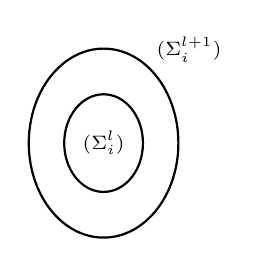
\begin{tikzpicture}
\draw[thick] (0,0) ellipse (0.95 and 1.2);
\draw[thick] (0,0) ellipse (0.5 and 0.62);
\node at (0,0) {\scriptsize $\Null(\Sigma_i^l)$};
\node[anchor=south west] at (0.55,0.9) {\scriptsize $\Null(\Sigma_i^{l+1})$};
\end{tikzpicture}
\end{minipage}\hfill
\begin{minipage}{0.65\textwidth}
\begin{align*}
x\in\Null(\Sigma_i^l)&\Rightarrow \Sigma_i^lx=0\\
&\Rightarrow \Sigma_i\cdot\Sigma_i^lx=\Sigma_i\cdot 0=0\\
&\Rightarrow \Sigma_i^{l+1}x=0\Rightarrow x\in\Null(\Sigma_i^{l+1})
\end{align*}
\end{minipage}

\begin{claim}
If $\Null(\Sigma_i^l)=\Null(\Sigma_i^{l+1})$ then $\Null(\Sigma_i^{l+1})=\Null(\Sigma_i^{l+2})$
% corrected: notes omitted "=" between the two null spaces
\end{claim}
Assume $\Null(\Sigma_i^l)=\Null(\Sigma_i^{l+1})$. Need to show $\Null(\Sigma_i^{l+1})=\Null(\Sigma_i^{l+2})$, i.e.
\begin{itemize}[itemsep=2pt,topsep=2pt]
\item[$\checkmark$] $\Null(\Sigma_i^{l+1})\subset\Null(\Sigma_i^{l+2})$
\item[] $\Null(\Sigma_i^{l+2})\subset\Null(\Sigma_i^{l+1})$
\end{itemize}
\begin{align*}
x\in\Null(\Sigma_i^{l+2})&\Rightarrow\Sigma_i^{l+2}x=0\\
&\Rightarrow \Sigma_i^{l+1}\,\Sigma_ix=0\Rightarrow\Sigma_ix\in\Null(\Sigma_i^{l+1})\\
&\Rightarrow\Sigma_ix\in\Null(\Sigma_i^l)\\
&\Rightarrow \Sigma_i^l\,\Sigma_ix=0\Rightarrow\Sigma_i^{l+1}x=0\Rightarrow x\in\Null(\Sigma_i^{l+1}) \qedhere
\end{align*}
\end{proof}
\begin{insight}[Consequence]
By the two claims the chain of null spaces grows strictly as long as it grows at all; once two consecutive null spaces coincide it is constant forever. Since the dimensions are bounded by $n$, the chain must stop growing, and it \key{stops exactly at the power $m_i$} (the exponent in $m(s)$), where the dimension equals the algebraic multiplicity $r_i$. Because each step adds at least one dimension, $m_i\le r_i$ again.
\end{insight}

\begin{example}
\[
A=\begin{bmatrix}
\boxed{\begin{smallmatrix}2&1&0\\0&2&1\\0&0&2\end{smallmatrix}} & & & & & \\
& \boxed{\begin{smallmatrix}2&1\\0&2\end{smallmatrix}} & & & & \\
& & \boxed{2} & & & \\
& & & \boxed{2} & & \\
& & & & \boxed{\begin{smallmatrix}3&1\\0&3\end{smallmatrix}} & \\
& & & & & \boxed{3}
\end{bmatrix}_{10\times10},
\qquad
\begin{aligned}
&\dim\Null\big((A-\lambda_iI)^l\big)=\,?\\
&d(s)=\,?\\
&m(s)=\,?
\end{aligned}
\]
\explain{Block diagonal; all entries outside the boxed blocks are zero.}

\paragraph{First block.}
\[
A_1=\bmat{2&1&0\\0&2&1\\0&0&2},\qquad d_1(s)=(s-2)^3,\qquad m_1(s)=(s-2)^3
\]
\begin{align*}
A_1-2I&=\bmat{0&1&0\\0&0&1\\0&0&0},\quad \rank=2, & \dim\Null(A_1-2I)&=1\\
(A_1-2I)^2&=\bmat{0&0&1\\0&0&0\\0&0&0}, & \dim\Null\big((A_1-2I)^2\big)&=2\\
(A_1-2I)^3&=\bmat{0&0&0\\0&0&0\\0&0&0}, & \dim\Null\big((A_1-2I)^3\big)&=3\\
(A_1-2I)^4&=0_{3\times3}, & \dim\Null\big((A_1-2I)^4\big)&=3\ \dots
\end{align*}
\explain{For $(A_1-2I)^3$: no need to calculate as it can be max 3 and is not equal to 1 or 2.}
% corrected: notes write "A" instead of "A_1" in the dimension column and in the last row
\explain{Each Jordan block of size $p$ behaves the same way: $\dim\Null\big((J-\lambda I)^l\big)=\min(l,p)$. Each block of $A$ contributes to the dimensions of $A$ independently.}

% ===== Page 67 =====
\needspace{14\baselineskip}
\paragraph{Whole matrix $A$.}\origpage{67}
\[
d(s)=(s-2)^7(s-3)^3
\]
\explain{$\lambda=2$ appears in blocks of sizes $3,2,1,1$ ($3+2+1+1=7$); $\lambda=3$ in blocks of sizes $2,1$ ($2+1=3$).}
\begin{align*}
&\Sigma_1=A-2I & &\Sigma_2=A-3I\\
&\dim\Null(\Sigma_1)=4 & &\dim\Null(\Sigma_2)=2\\
&\dim\Null(\Sigma_1^2)=6 \quad(+2) & &\dim\Null(\Sigma_2^2)=3 \quad(+1)\\
&\dim\Null(\Sigma_1^3)=7 \quad(+1) & &\Rightarrow (s-3)^2 \quad(+0)\\
&\Rightarrow (s-2)^3 \quad(+0)
\end{align*}
\[
\boxed{\therefore\ m(s)=(s-2)^{3}(s-3)^{2}}
\]
\explain{Exponent 3: largest Jordan block (JB) for $\lambda_i=2$;\quad exponent 2: largest JB for $\lambda_i=3$.}
\end{example}

\subsection{Counting Jordan Blocks}\label{ss:counting-jb}
(JB: Jordan block.)
\begin{align*}
\dim\Null(\Sigma_i)&=\#\text{ of JB's for }\lambda_i\\
&=\#\text{ of JB's with size}\ge1\text{ for }\lambda_i\\
&=\max\#\text{ of linearly independent eigenvectors for }\lambda_i
\end{align*}
\begin{align*}
\dim\Null(\Sigma_i^2)-\dim\Null(\Sigma_i^1)&=\#\text{ of JB's with size}\ge2\text{ for }\lambda_i\\
\dim\Null(\Sigma_i^3)-\dim\Null(\Sigma_i^2)&=\#\text{ of JB's with size}\ge3\text{ for }\lambda_i\\
&\;\;\vdots\\
\dim\Null(\Sigma_i^{l})-\dim\Null(\Sigma_i^{l-1})&=\#\text{ of JB's with size}\ge l\text{ for }\lambda_i.
\end{align*}
% corrected: notes had dim N(Sigma^{l+1}) - dim N(Sigma^l) = # JB's with size >= l (off by one);
% shifted indices so that the case l=1 below is the first line
For $l=1$:
\[
\dim\Null(\Sigma_i)-\underbrace{\dim\Null\big(\overbrace{\Sigma_i^0}^{I}\big)}_{0}=\#\text{ of JB's with size}\ge1\text{ for }\lambda_i
\]
\explain{Works for $l=1$ also.}

\key{$m_i$ is the size of the largest JB.}
\begin{insight}[Reading off the block sizes]
Write $\delta_l=\dim\Null(\Sigma_i^l)-\dim\Null(\Sigma_i^{l-1})$ (the increments, $\delta_l=\#$ JB's of size $\ge l$). Then
\[
\#\text{ of JB's of size exactly } l \;=\; \delta_l-\delta_{l+1}.
\]
Reason: a block of size $p$ contributes $1$ to $\dim\Null(\Sigma_i^l)$ for each $l\le p$, so it raises the dimension by one at each of the steps $l=1,\dots,p$ and not after. The increments therefore stop being positive at $l=m_i$, the size of the largest block.
\end{insight}

\sep
\needspace{10\baselineskip}
$\Rightarrow$ For diagonalizable matrix, minimal polynomial should have the power at most 1:
\begin{keybox}
\centering JCF is diagonal iff $m_i=1\ \forall i$
\end{keybox}
\begin{align*}
\C^n&=\Null(\Sigma_1^{m_1})\oplus\cdots\oplus\Null(\Sigma_k^{m_k})\\
\C^n&=\underbrace{\Null(\Sigma_1)}_{r_1}\oplus\cdots\oplus\underbrace{\Null(\Sigma_k)}_{r_k}
\end{align*}
\explain{$\Null(\Sigma_1)$: at most $r_1$ linearly independent eigenvectors.}
The second decomposition holds exactly when $m_i=1$ for all $i$, i.e.\ when $\dim\Null(\Sigma_i)=r_i$ for every eigenvalue.

$\Rightarrow$ \key{$A$ is diagonalizable iff there exist $n$ linearly independent eigenvectors for $A$.}

% ===== Page 68 =====
\begin{example}
\leavevmode\origpage{68}\[
A=\bmat{1&-1&1&0\\1&-1&0&0\\0&0&0&0\\2&-2&-2&0}
\quad\Rightarrow\quad
\begin{aligned}
&d(s)=s^4\\
&m(s)=\,?\\
&\text{JCF}=\,?
\end{aligned}
\]
\explain{$d(s)=s^4$: Learn to calculate this! (Shortcut: $A^3=0$ below, so every eigenvalue satisfies $\lambda^3=0$, i.e.\ $\lambda=0$ with multiplicity 4.)}
\begin{align*}
\Sigma_1&=A-\cancel{\lambda_1}^{\,0}I=A, &
\dim\Null(\Sigma_1)&=2, \quad \dim\Null(\Sigma_1^2)=3, \quad \dim\Null(\Sigma_1^3)=4
\end{align*}
\[
A^2=\bmat{0&0&1&0\\0&0&1&0\\0&0&0&0\\0&0&2&0},\qquad
A^3=\bmat{0&0&0&0\\0&0&0&0\\0&0&0&0\\0&0&0&0}
\]
\explain{$\rank A=2$ (row 4 $=-2\cdot$row 1$+4\cdot$row 2, row 3 $=0$) $\Rightarrow\dim\Null(A)=2$; $\rank A^2=1\Rightarrow\dim\Null(A^2)=3$; $A^3=0\Rightarrow\dim\Null(A^3)=4$.}
\begin{align*}
&\therefore\ m(s)=s^3\\
&\#\text{ of JB's}=2 &&(2-0)\\
&\#\text{ of JB's with size}\ge2=1 &&(3-2)\\
&\#\text{ of JB's with size}\ge3=1 &&(4-3)\\
&\#\text{ of JB's with size}\ge4=0 &&(4-4)
\end{align*}
$\Rightarrow$ one JB with size $=3$, zero JB with size $=2$, one JB with size $=1$:
\[
\text{JCF}=\left[\begin{array}{ccc|c}0&1&0&0\\0&0&1&0\\0&0&0&0\\\hline0&0&0&0\end{array}\right]
\]
$\Rightarrow$ \key{Not diagonalizable!} Only $\dim\Null(A)=2<4$ independent eigenvectors exist; equivalently, $m_1=3\neq1$.
\end{example}

\needspace{12\baselineskip}
\begin{example}
Let $A\in\R^{8\times8}$ have the following subspace dimensions:
\begin{alignat*}{2}
\dim\Null(A-3I)&=5 &\qquad& (+5)\\
\dim\Null\big((A-3I)^2\big)&=7 && (+2)\\
\dim\Null\big((A-3I)^3\big)&=8 && (+1)\\
& && (+0)
\end{alignat*}
$d(s)=\,?$\quad $m(s)=\,?$\quad $\text{JCF}=\,?$
\begin{align*}
m(s)&=(s-3)^3\\
d(s)&=(s-3)^8
\end{align*}
\explain{$\Rightarrow$ the maximum number of linearly independent eigenvectors is 5.}
\explain{$\dim\Null\big((A-3I)^3\big)=8=n$, so $3$ is the only eigenvalue ($r_1=8$) and the chain stops at power $3$ ($m_1=3$).}
Block sizes from the increments $5,2,1,0$: \ $5$ JB's in total; $5-2=3$ of size $1$, $2-1=1$ of size $2$, $1-0=1$ of size $3$ \ (check: $3\cdot1+1\cdot2+1\cdot3=8$).
\[
\text{JCF}=\left[\begin{array}{ccc|cc|c|c|c}
3&1&0&0&0&0&0&0\\
0&3&1&0&0&0&0&0\\
0&0&3&0&0&0&0&0\\\hline
0&0&0&3&1&0&0&0\\
0&0&0&0&3&0&0&0\\\hline
0&0&0&0&0&3&0&0\\\hline
0&0&0&0&0&0&3&0\\\hline
0&0&0&0&0&0&0&3
\end{array}\right]
\]
\end{example}

\begin{example}
Let $A\in\R^{4\times4}$. Single eigenvalue at $\lambda=7$, $m_1=2$. Find all possible JCFs the matrix $A$ can have.
\begin{align*}
d(s)&=(s-7)^4\\
m(s)&=(s-7)^2
\end{align*}
\[
\begin{array}{ccc}
\Null(A-7I) & \subsetneq & \Null\big((A-7I)^2\big)\\
1\le\ \ ? & & 4\\
\scriptstyle \dim=2\text{ or }3\text{ or }1 & &
\end{array}
\]
% (example continues on page 69 -- closed in part7)
